\section{组件}
\subsection{组件布局}
\indent\urwid{} 利用组件分割屏幕空间. 使得实现动态的界面十分容易, 可以适应不同的终端和字体大小. \cref{fig:example_of_widget_layout} 是一个 \urwid{} 布局的例子.%
%
\begin{figure}[!htb]
    \centering
    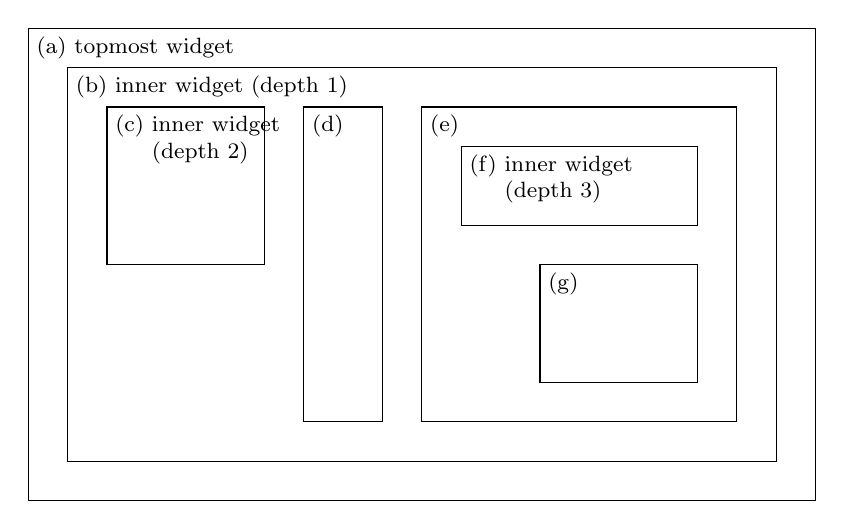
\begin{tikzpicture}[
  block/.style = {rectangle, draw},
  number/.style = {anchor = north west, inner sep = 3pt, font = \footnotesize, align = flush left}
]
  \node[block, minimum width = 10cm, minimum height = 6cm]   (a) at (5,   5.5)  {};
  \node[block, minimum width = 9cm,  minimum height = 5cm]   (b) at (5,   5.5)  {};
  \node[block, minimum width = 2cm,  minimum height = 2cm]   (c) at (2,   6.5)  {};
  \node[block, minimum width = 1cm,  minimum height = 4cm]   (d) at (4,   5.5)  {};
  \node[block, minimum width = 4cm,  minimum height = 4cm]   (e) at (7,   5.5)  {};
  \node[block, minimum width = 3cm,  minimum height = 1cm]   (f) at (7,   6.5)  {};
  \node[block, minimum width = 2cm,  minimum height = 1.5cm] (g) at (7.5, 4.75) {};
  
  \node[number] at (a.north west) {(a) topmost widget};
  \node[number] at (b.north west) {(b) inner widget (depth 1)};
  \node[number] at (c.north west) {(c) inner widget\\\hphantom{(c) }(depth 2)};
  \node[number] at (d.north west) {(d)};
  \node[number] at (e.north west) {(e)};
  \node[number] at (f.north west) {(f) inner widget\\\hphantom{(f) }(depth 3)};
  \node[number] at (g.north west) {(g)};
\end{tikzpicture}
    \caption{\urwid{} 布局举例}
    \label{fig:example_of_widget_layout}
\end{figure}%
%
组件的渲染会适应屏幕的大小, 当渲染最前面的组件时:%
%
\begin{itemize}
  \item 组件 (a) 全屏渲染.
  \item 在组件 (a) 上渲染组件 (b) 时, 是全屏渲染.
  \item 在组件 (b) 上渲染组件 (c), (d), (e) 时, 会将显示区域分割成三列.
  \item 在组件 (e) 上渲染最近 (f), (g) 时, 会将显示区域分割成两行.
  \item 组建 (e) 将组件 (f) 和 (g) 组合后一起返回.
  \item 组件 (b) 将组件 (c), (d) 和 (e) 组合后一起返回.
  \item 组件 (a) 与组件 (b) 组合, 并返回.
\end{itemize}%
%
组件 (a), (b) 和 (e) 被称为容器, 因为他们可以承载其它组件. 容器决定了其包含的组件的大小和位置. 容器必须跟踪当前的焦点组件. 在\cref{fig:example_of_widget_layout} 
中, 组件 (e) 的焦点组件是组件 (f), 同样, 组件 (e) 也是 (b) 的焦点组件. 如果组件 (f) 是一个文本框, 那么用户的输入将按照如下方式处理.%
%
\begin{itemize}
  \item 组件 (a) 将按键信息传给焦点组件 (b).
  \item 组件 (b) 将按键信息传给焦点组件 (e).
  \item 组件 (e) 将按键信息传给焦点组件 (f).
  \item 组件 (f) 要么处理按键, 要么直接返回这个按键信息.
  \item 如果组件 (f) 返回按键信息, 则组件 (e) 要么处理按键, 要么直接返回这个按键信息.
  \item 如果组件 (e) 返回按键信息, 则组件 (b) 要么处理按键, 要么直接返回这个按键信息.
  \item 如果组件 (b) 返回按键信息, 则组件 (a) 处理按键信息.
\end{itemize}
